\chapter{Análisis de una señal AM}
Utilizando dos generadores de señales, se creó una señal
modulada en AM de $200 \si{\milli\volt}pp$ donde:

Frecuencia de la portadora: $900 \si{\kilo\hertz}$.

Frecuencia de la moduladora: $100 \si{\kilo\hertz}$.

Luego, con el analizador de espectros, y simulando el espectro
de la señal en MATLAB, se verificaron las señales medidas. Además, se
utilizó un osciloscopio en paralelo para verificar las amplitudes
de las señales.

\begin{enumerate}
    \item Moduladora Senoidal; $m=0.5$
    \item Moduladora Senoidal; $m=1$
    \item Moduladora Triangular; $m=1$
    \item Moduladora Senoidal; $m=1$; frecuencia igual a la portadora
\end{enumerate}

\begin{figure}[ht]
    \begin{center}
        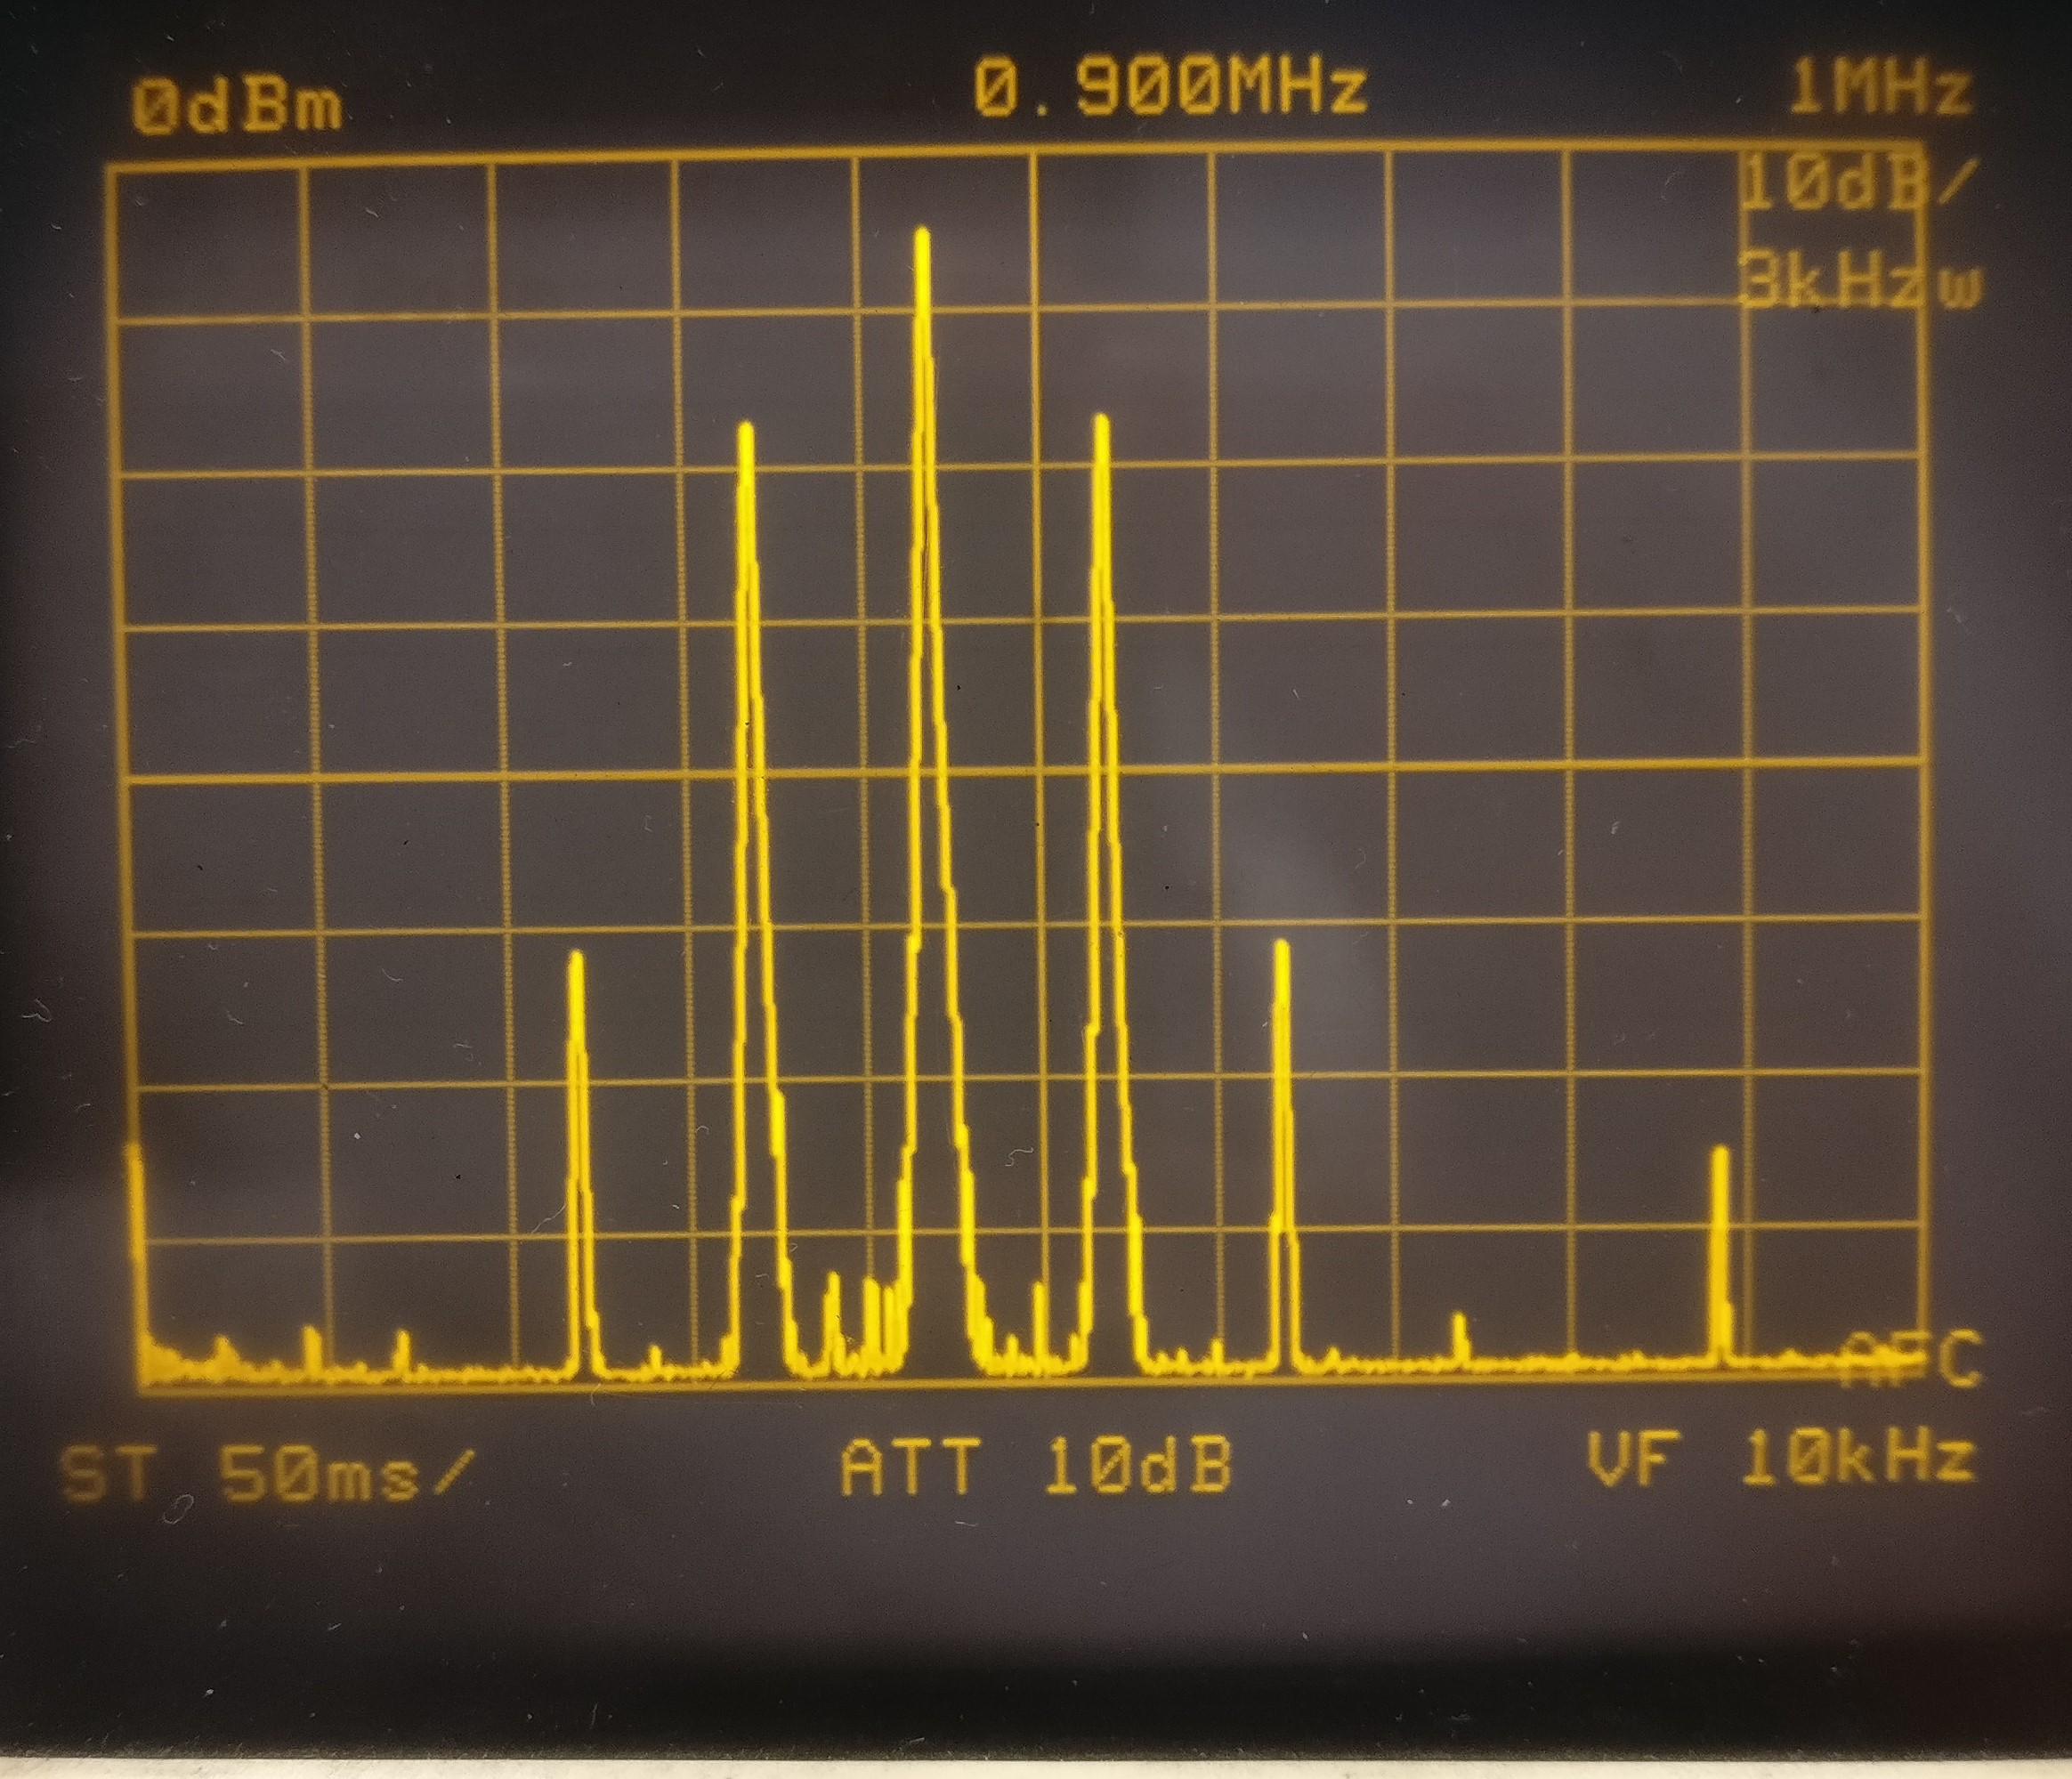
\includegraphics[width=0.6\linewidth]{contenido/img/espectro_am05.jpg}
        \caption{Espectro de la señal modulada con senoidal y m = 0.5}
        \label{fig:am:05}
    \end{center}
\end{figure}

\begin{figure}[ht]
    \begin{center}
        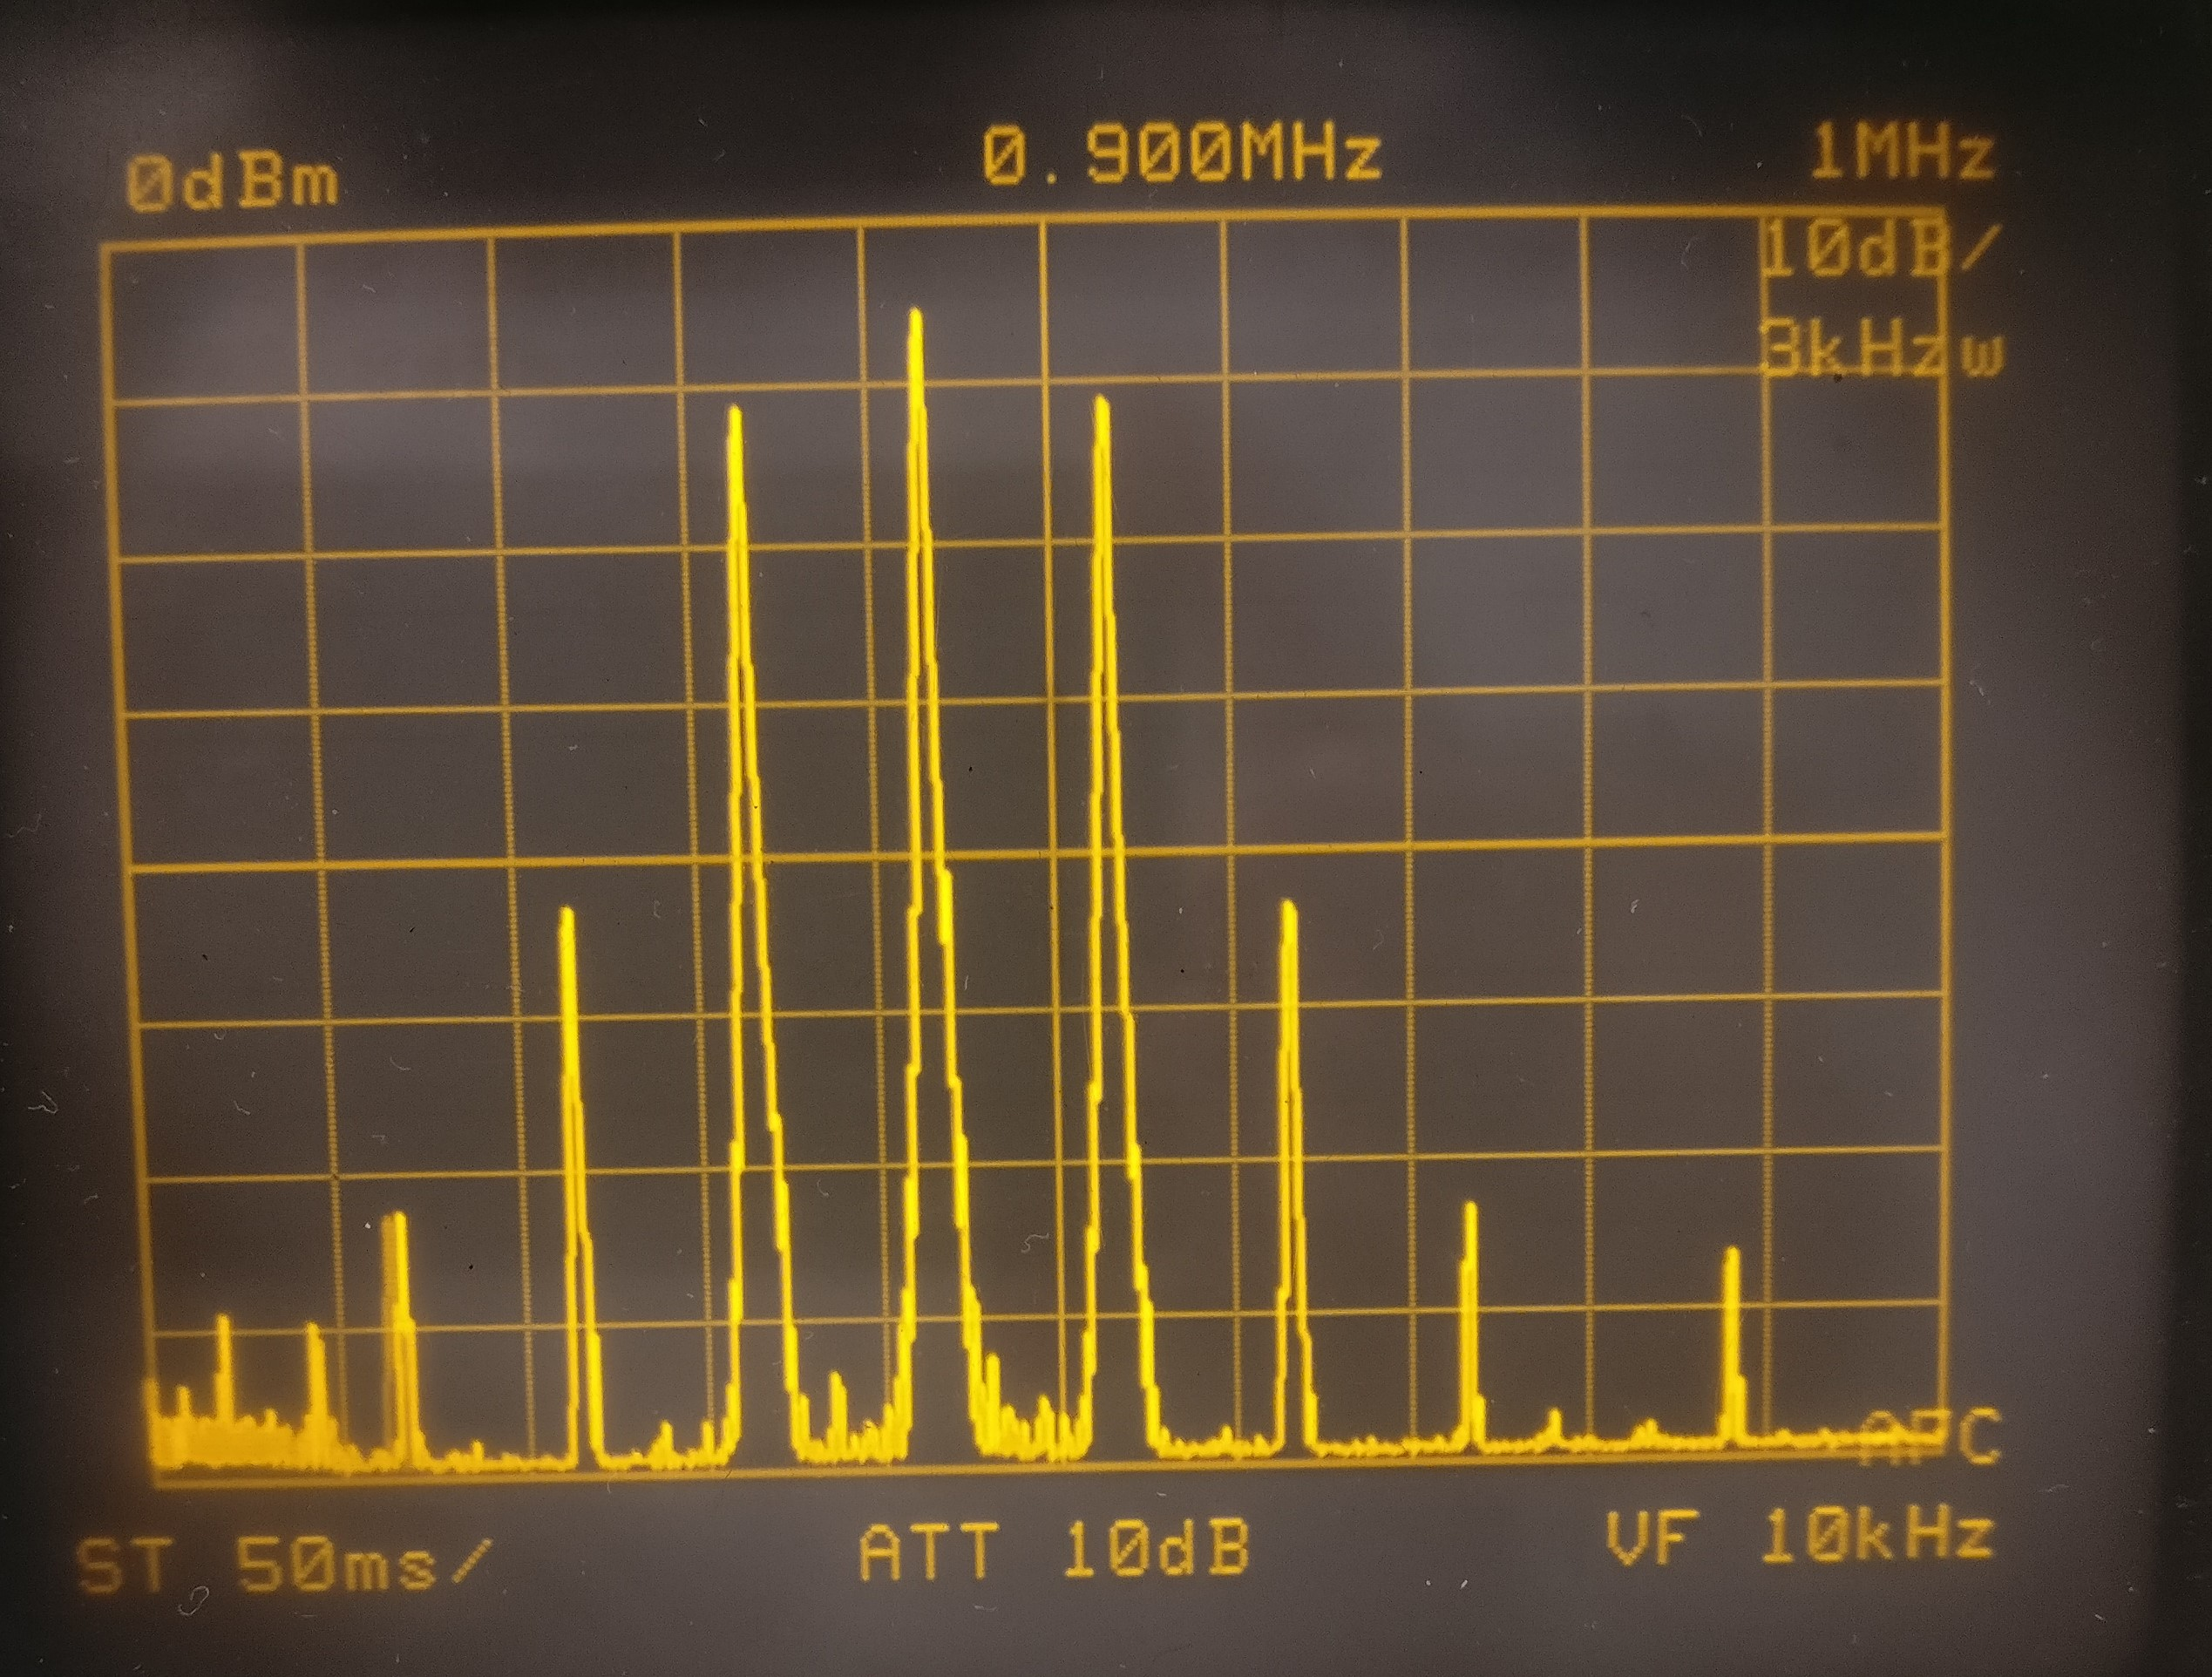
\includegraphics[width=0.6\linewidth]{contenido/img/espectro_am1.jpg}
        \caption{Espectro de la señal modulada con senoidal y m = 1}
        \label{fig:am:1}
    \end{center}
\end{figure}

Como se observa de las figuras \ref{fig:am:05} y \ref{fig:am:1}, está presente,
en el centro de las potencias observadas, la potencia de la señal portadora, y a
sus lados las potencias de las señales resultantes de la modulación.